\documentclass{article}
\usepackage[T2A]{fontenc} 
\usepackage[utf8]{inputenc} 
\usepackage[english,russian]{babel}
\usepackage{graphicx} 
\usepackage{amsmath}
\usepackage{amsfonts} 
\usepackage{titlesec}
\usepackage{listings}
\usepackage{float}
\usepackage{longtable}
\usepackage{titling} 
\usepackage{geometry} 
\usepackage{pgfplots}
\pgfplotsset{compat=1.9}
\usepackage{xcolor}
\definecolor{darkgreen}{RGB}{0,100,0}

\lstset{
  language=Python,
  basicstyle=\ttfamily,
  keywordstyle=\color{darkgreen},
  stringstyle=\color{purple},
  commentstyle=\color{green},
  morecomment=[l][\color{magenta}]{\#},
  frame=single, 
  showspaces=false, 
  showstringspaces=false, 
  numbers=left, 
  numberstyle=\tiny,
}

\titleformat{\section}
  {\normalfont\Large\bfseries}{\thesection}{1em}{}
\titleformat{\subsection}
  {\normalfont\large\bfseries}{\thesubsection}{1em}{}

\setlength{\droptitle}{-6em} 
\title{Отчет по лабораторной работе № 7\\ Вариант № 3}
\author{Винницкая Дина Сергеевна}
\date{Группа: Б9122-02-03-01сцт}

\geometry{a4paper, margin=2cm}

\begin{document}

\maketitle
\section*{Цель работы}
\begin{enumerate}
    \item Определить примерный интервал в котором может располагаться необходимый корень
    \item Численно найти решение тремя известными методами
    \item Сформировать сравнительную таблицу, отражающую сходимость методов 
    \item Сделать вывод о проделанной работе 

    
\end{enumerate}

\section*{Входные данные:}
\begin{enumerate}

    \item \textbf{Уравнение:} $ 0 = 2^x - 2x^2 - 1$


\end{enumerate}

\section*{\text{Определение области рассмотрения}}
Для функции $2^x - 2x^2 - 1$ необходимо определить область рассмотрения, учитывая особенности экспоненциальной и полиномиальной функций.
$$\textbf{Определение области рассмотрения}$$
\begin{itemize}
    \item Для начала, исследуем корни полинома. Простейший способ найти корень полинома - это приравнять его к нулю и решить полученное уравнение. В данном случае, уравнение можно численно решить, и находится, что корень приблизительно равен 1.44.
    \item Поскольку полином третьей степени быстро возрастает, а экспонента быстро убывает в положительной области, положительный корень уравнения находится не сильно дальше от 1.44.
    \item Следовательно, пока что возьмем промежуток [0,3, 1,5] для определения области рассмотрения функции.
\end{itemize}
$$\textbf{Отрицательный корень}$$
\begin{itemize}
    \item Также существует еще один корень уравнения, который находится в отрицательной области. В этой области полином третьей степени стремительно уходит в отрицательную бесконечность. Однако, учитывая свойства показательной функции, можно сделать вывод о том, что где-то существует и отрицательный корень, но в данной ситуации поиск его не представляется необходимым
\end{itemize}
\section*{\text{Реализация методов}}

\textbf{\large{Метод Хорд}} \\
    Это численный метод для приближенного нахождения корня нелинейного уравнения. Он основан на идее использования хорды (отрезка, соединяющего две точки на графике функции), чтобы приблизиться к корню.
\begin{figure}[H]
    \centering
    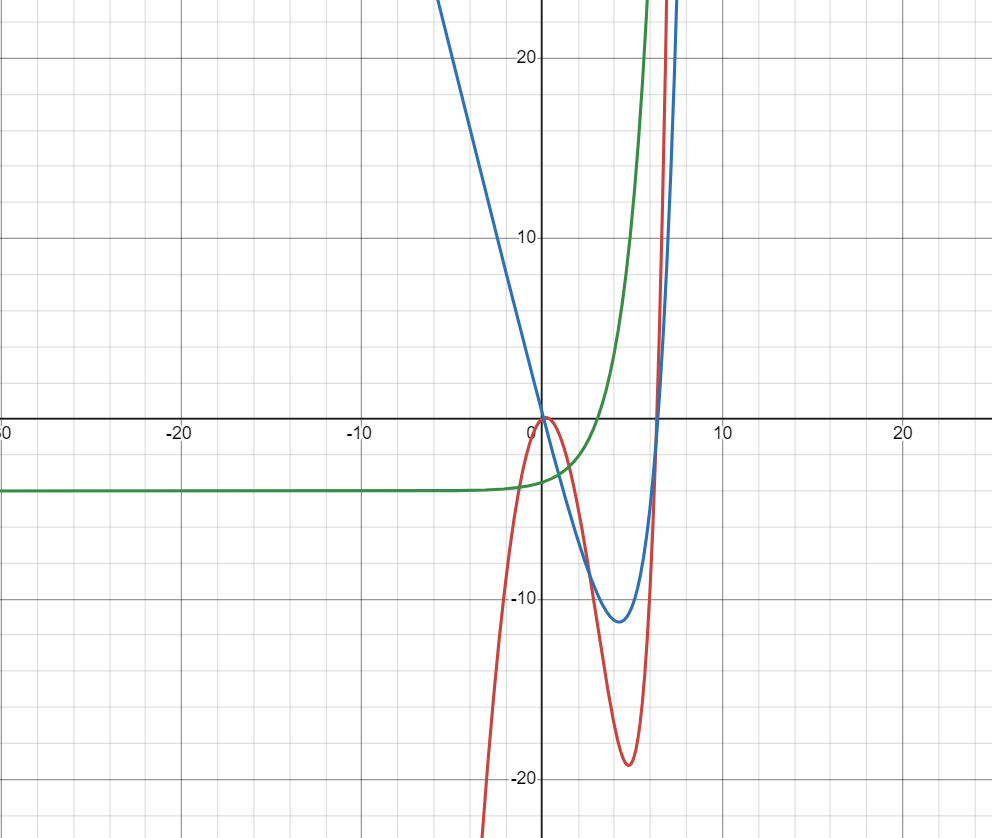
\includegraphics[width=\textwidth]{lab_7_1.png}
    \label{fig:my_label}
    \caption{График функции и ее первой и второй производной}
\end{figure}
\begin{lstlisting}
def chord_method(eps, lst: list):
    table = PrettyTable()
    counter = 1
    b = lst[1]
    x_prev = lst[0]
    x_next = x_prev - (b - x_prev) * function(x_prev) 
    / (function(b) - function(x_prev))
    table.add_row([counter, x_next])

    while abs(x_next - x_prev) > eps:
        x_prev = x_next
        x_next = x_prev - (b - x_prev) * function(x_prev) 
        / (function(b) - function(x_prev))
        counter += 1
        table.add_row([counter, x_next])

    print(table.get_string(border=True, header=False, hrules=1))
    return x_next

\end{lstlisting}

$$\textbf{Обозначения}$$
\begin{itemize}
    \item eps - значение погрешности, используемое для остановки итераций (то есть критерий остановки метода).
    \item lst - список значений, представляющих начальный отрезок для метода.
    \item counter - переменная, отвечающая за отслеживание количества итераций.
    \item b - второй элемент списка lst.
   \item x\_prev - первый элемент списка lst.
   \item x\_next - вычисляемое следующее приближение корня уравнения
\end{itemize}
$$\textbf{Алгоритм}$$
\begin{enumerate}
    \item Вычисляется новое значение x\_next на основе текущего приближения x\_prev и значения функции в точке x\_prev.
    \item Затем проверяется условие остановки: (|x\_{\text{next}} - x\_{\text{prev}}| > \text{eps}).
    \item Если условие не выполнено, то происходит обновление x\_prev, вычисление нового x\_next и увеличение счетчика итераций.
    \item После завершения итераций выводится таблица с результатами итераций, сгенерированная с помощью метода get\_string объекта table.
    \item Наконец, возвращается последнее найденное значение x\_next, которое является приближенным значением корня уравнения.
\end{enumerate}

$$\textbf{Таблица значений}$$

\begin{table}[h!]
\centering
\begin{tabular}{|c|c|c|c|}
\hline
Итерация & Значение & Итерация & Значение \\
\hline
1 & 0.322541193046703 & 21 & 0.3991525127269086 \\
\hline
2 & 0.3409645084710158 & 22 & 0.39918859088335995 \\
\hline
3 & 0.3555675656565128 & 23 & 0.39921452106708516 \\
\hline
4 & 0.36686352496279695 & 24 & 0.3992331568543878 \\
\hline
5 & 0.3754373981027205 & 25 & 0.3992465498018522 \\
\hline
6 & 0.3818520031969649 & 26 & 0.39925617466842017 \\
\hline
7 & 0.3865995358189016 & 27 & 0.39926309148370676 \\
\hline
8 & 0.39008519745005094 & 28 & 0.39926806212635957 \\
\hline
9 & 0.3926293522424672 & 29 & 0.3992716341575618 \\
\hline
10 & 0.3944783323328586 & 30 & 0.3992742010951745 \\
\hline
11 & 0.3958178893602863 & 31 & 0.3992760457431182 \\
\hline
12 & 0.3967861773641209 & 32 & 0.3992773713364518 \\
\hline
13 & 0.39748494883616114 & 33 & 0.3992783239267496 \\
\hline
14 & 0.3979886248743356 & 34 & 0.39927900847063347 \\
\hline
15 & 0.3983513657463251 & 35 & 0.39927950039227667 \\
\hline
16 & 0.398612446298662 & 36 & 0.3992798538929168 \\
\hline
17 & 0.39880027425661835 & 37 & 0.3992801079224546 \\
\hline
18 & 0.3989353593985572 & 38 & 0.3992802904708603 \\
\hline
19 & 0.39903248985084655 & 39 & 0.3992804216521015 \\
\hline
20 & 0.3991023181845276 & 40 & 0.3992805159203268 \\
\hline
\end{tabular}
\caption{Значения итераций метода Хорд}
\end{table}


\begin{figure}[H]
    \centering
    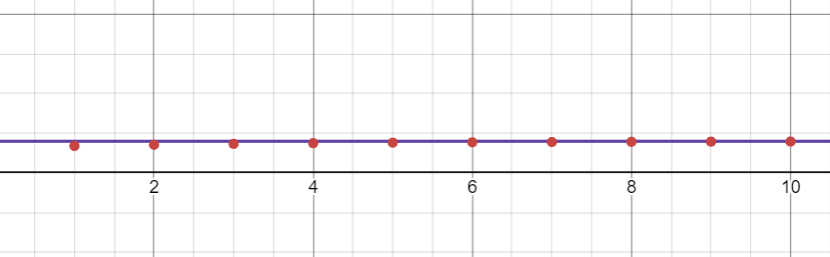
\includegraphics[width=\textwidth]{lab_7_2.png}
    \caption{График значений}
    \label{fig:my_label}
\end{figure}

\begin{itemize}
    \item Как можно заметить из представленного графика - метод сходится к 9 итерации
\end{itemize} 

\textbf{\large{Метод Ньютона}} 
\begin{lstlisting}
def newton_method(eps, x0):
    table = PrettyTable()
    count = 1
    x_prev = x0
    x_next = x_prev - function(x_prev) / derivative_function(x_prev)
    table.add_row([count, x_next])
    
    while abs(x_next - x_prev) > eps:
        count += 1
        x_prev = x_next
        x_next = x_prev - function(x_prev) / derivative_function(x_prev)
        table.add_row([count, x_next])
    print(table.get_string(border=True, header=False, hrules=1))
    return x_next

\end{lstlisting}
$$\textbf{Обозначения}$$
\begin{itemize}
    \item eps - значение погрешности, используемое для остановки итераций (критерий остановки метода).
    \item x0 - начальное приближение для корня.
    \item count - переменная, отслеживающая количество итераций.
    \item x\_prev - предыдущее приближение.
    \item x\_next - вычисляемое следующее приближение корня уравнения на основе предыдущего значения и значений функции и её производной.

\end{itemize}

$$\textbf{Алгоритм}$$
\begin{enumerate}
    \item Выбирается начальное приближение \( x_0 \).
    \item Вычисляется следующее приближение по формуле:
    \[
    x_{n+1} = x_n - \frac{f(x_n)}{f'(x_n)}
    \]
    \item Процесс повторяется до тех пор, пока разница между последовательными приближениями не станет меньше заданной точности \( \epsilon \).
\end{enumerate}

$$\textbf{Значения}$$
\begin{table}[H]
\centering

\begin{tabular}{|c|c|}
\hline
Итерация & Значение \\
\hline
1 &  0.8386350669976804 \\
\hline
2 &  0.5463059242914783 \\
\hline
3 & 0.42988681718031907 \\
\hline
4 &  0.401281869581121  \\
\hline
5 & 0.39929052760214123 \\
\hline
6 &  0.3992807568969161 \\
\hline
7 &  0.3992807566616375 \\
\hline
\end{tabular}
\caption{Значения итераций метода Ньютона}
\end{table}
$$\textbf{Сходимость}$$
\begin{figure}[H]
    \centering
    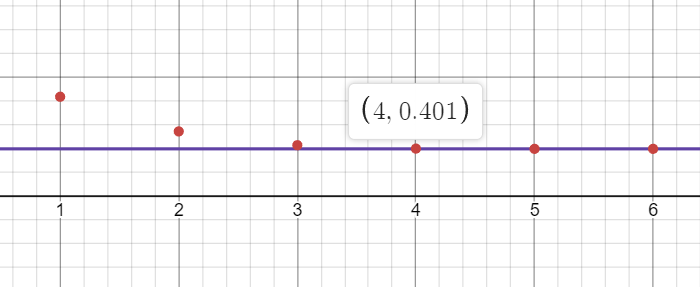
\includegraphics[width=\textwidth]{lab_7_3.png}
    \caption{График сходимости}
    \label{fig:my_label}
\end{figure}
\begin{itemize}
    \item Как можно заметить, метод Ньютона сходится к 4 итерации.
\end{itemize}
\textbf{\large{Метод Бисекции}} 
Метод бисекции (или метод деления пополам) — это численный метод для нахождения корней уравнений вида \( f(x) = 0 \). Этот метод требует, чтобы функция \( f(x) \) была непрерывной на интервале \([a, b]\) и чтобы значения функции на концах этого интервала имели разные знаки (т.е., \( f(a) \) и \( f(b) \) должны иметь противоположные знаки).
\begin{lstlisting}
def bisection_method(eps, lst: list):
    l = lst[0]
    r = lst[1]
    c = 0
    count = 1
    x_prev = r
    x_next = c
    while abs(x_next - x_prev) > eps:
        c = (r + l) / 2
        if function(c) * function(l) > 0:
            l = c
        elif function(c) * function(r) > 0:
            r = c
        x_prev = x_next
        x_next = c
        print(count, x_next)
        count += 1
    return x_next

\end{lstlisting}


$$\textbf{Обозначения}$$
\begin{itemize}
    \item ps - значение погрешности, используемое для остановки итераций (то есть критерий остановки метода).
    \item lst - список значений, представляющих начальный отрезок для метода.
    \item l - левый конец начального отрезка.
    \item r - правый конец начального отрезка.
    \item c - середина отрезка.
    \item count - переменная, отвечающая за отслеживание количества итераций.
    \item x\_prev и x\_next - переменные для хранения предыдущего и следующего приближенных значений корня.
\end{itemize}

$$\textbf{Алгоритм}$$

\begin{enumerate}
    \item Выбирается начальный интервал \([a, b]\), в котором функция меняет знак.
    \item Вычисляется середина интервала \( c = \frac{a + b}{2} \).
    \item Проверяется знак функции в точке \( c \):
    \begin{itemize}
        \item Если \( f(c) \) имеет тот же знак, что и \( f(a) \), то \( c \) становится новой левой границей интервала.
        \item Если \( f(c) \) имеет тот же знак, что и \( f(b) \), то \( c \) становится новой правой границей интервала.
    \end{itemize}
    \item Процесс повторяется до тех пор, пока длина интервала не станет меньше заданной точности \( \epsilon \).
\end{enumerate}

$$\textbf{Значения}$$
\begin{table}[h!]
\centering
\begin{tabular}{|c|c|c|c|}
\hline
Итерация & Значение & Итерация & Значение \\
\hline
1 & 1.0 & 13 & 1.4998779296875 \\
\hline
2 & 1.25 & 14 & 1.49993896484375 \\
\hline
3 & 1.375 & 15 & 1.499969482421875 \\
\hline
4 & 1.4375 & 16 & 1.4999847412109375 \\
\hline
5 & 1.46875 & 17 & 1.4999923706054688 \\
\hline
6 & 1.484375 & 18 & 1.4999961853027344 \\
\hline
7 & 1.4921875 & 19 & 1.4999980926513672 \\
\hline
8 & 1.49609375 & 20 & 1.4999990463256836 \\
\hline
9 & 1.498046875 & 21 & 1.4999995231628418 \\
\hline
10 & 1.4990234375 & 22 & 1.499999761581421 \\
\hline
11 & 1.49951171875 & 23 & 1.4999998807907104 \\
\hline
12 & 1.499755859375 & 24 & 1.4999999403953552 \\
\hline
\end{tabular}
\caption{Значения итераций метода Бисекций}
\end{table}


$$\textbf{Сходимость}$$
\begin{figure}[H]
    \centering
    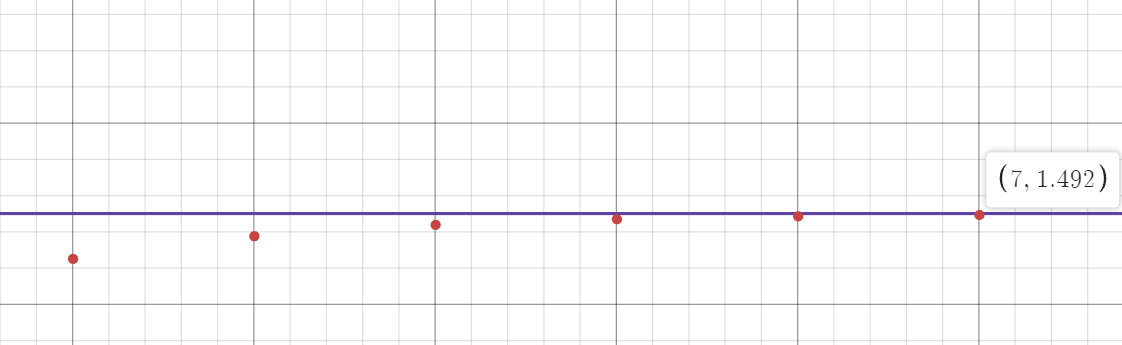
\includegraphics[width=\textwidth]{lab_7_4.png}
    \caption{График сходимости}
    \label{fig:my_label}
\end{figure}
\begin{itemize}
    \item Исходя из приведенного графика можно сделать вывод о том, что метод бисекции сходится к 7 итерации
\end{itemize}
\section*{Заключение}
В результате проделанной работы можно сделать ряд выводов:
\begin{enumerate}
    \item Метод хорд сходится за 9 итераций, метод Ньютона за 4, а метод бисекций за 7.
    \item Таким образом, в результате проделанной работы и анализу методов можно сделать вывод о том, что в данном случае метод Ньютона сошелся быстрее всех, а именно за 4 итерации.
    \item В ходе экспериментов использовалась функция \( f(x) = 2^x - 2x^2 - 1 \) с начальными условиями \( x_0 = 1 \) для метода Ньютона и интервалом \([0.5, 2]\) для метода бисекций.
    \item Вычислительная точность была задана как \( \epsilon = 10^{-6} \), что обеспечило необходимую точность результатов.
    \item Метод Ньютона показал наивысшую эффективность и быструю сходимость.
    \item Метод хорд не требует вычисления производной, но может сходиться медленнее в зависимости от выбора начальных точек.
    \item Метод бисекций является надежным и простым в реализации, но может потребовать больше итераций для достижения требуемой точности.
   
\end{enumerate}



\end{document}

